\documentclass[10pt]{article}

\usepackage{parskip}
\usepackage[margin=1in]{geometry} 
\usepackage{tikz}
\usetikzlibrary{positioning}
\usepackage{amsmath,amsthm,amssymb, graphicx, multicol, array}
\usepackage{enumitem}
\usepackage{amssymb}
\usepackage{float}
\usepackage{href-ul}
 
\newcommand{\N}{\mathbb{N}}
\newcommand{\Z}{\mathbb{Z}}
 
\newenvironment{problem}[2][Problem]{\begin{trivlist}
\item[\hskip \labelsep {\bfseries #1}\hskip \labelsep {\bfseries #2.}]}{\end{trivlist}}

\begin{document}
 
\title{Matching \& weighting}
\author{Jakob Sverre Alexandersen\\
GRA4158 Marketing and the Analysis of Experiments and Quasi-Experiments\\
Lecture 9}
\maketitle

\tableofcontents
\newpage
\section{Recap: conditional independence / covariate adjustment}
\begin{itemize}
    \item Can treatment allocation be randomized? -- No
    \item Time series available? -- No 
    \item Covariates available? -- Yes
    \item Regression adjustment 
    \item Matching and weighting
    \item Double ML 
    \item Core assumptions: conditional independence / unconfoundedness
\end{itemize}
\subsection{Non-random assignment -- quasi-experimental methods}
\begin{itemize}
    \item We have non-random assignment $\to $ there are selection effects:
    \begin{itemize}
        \item \textbf{Selection on unobservables}
        \begin{itemize}
            \item We do not have sufficient covariates to capture the selection mechanism
            \item Focal treatment effect correlates with the unobserved error because of these omitted variables / confounders (i.e., endogeneity bias, confounder bias)
            \item Instrumental variable methods 
            \item IV-free methods 
        \end{itemize}
        \item \textbf{Selection on observables}
        \begin{itemize}
            \item We have ALL necessary covariates to capture the selection mechanism
            \item \textbf{Conditional independence} -- when we sufficiently control for the influence of the covariates, we achieve independence / unconfoundedness of the treatment variable
            \item Regression adjustment, matching and weighting
            \item Double ML 
        \end{itemize}
    \end{itemize}
\end{itemize}
\subsection{Recap: non-random assignment}
\begin{itemize}
    \item We do not have random assignment (i.e., independence of potential outcomes from treatment $\{Y_i(1), Y_i(0) \bot T_i\}$)

    but we assume conditional independence: $\{Y_i(1), Y_i(0)\} \bot T_i|X_i$
    \item In lec 2, we have learned that OLS regression can identify ATE by controlling for $X $
    \begin{itemize}
        \item However, there are some problems with OLS: it is linear, parametric, and does a variance weighting
    \end{itemize}
    \item We want to look at other ways of estimating treatment effects (i.e., ATE, ATET) relying on the principle of estimating treatment effects for individuals that are equal on $X $
\end{itemize}
\textbf{Data rich environments}: many of the following methods are especially popular in data-rich environments, like online advertising. We have a massive feature / covariate space. They typically assume that we have a high-dimensional covariate matrix (many covariates). Traditional linear regression is good when focusing on a few theoretically well justified vairables and mainly linear influences (or specific non-linear or interaction terms): it struggles to control for hundreds of complex, interacting variables without overfitting. 
\newpage 
\section{Core idea of matching}
\textbf{Situation}
\begin{itemize}
    \item A (set of) confounding variable(s) $X $ assign individuals to treatment and control so that these two groups are initially not comparable in their potential outcomes 
\end{itemize}
\textbf{Idea}
\begin{itemize}
    \item We want to pair treated units with an equal/similar untreated unit to achieve a new sample that is comparable
    \item We want to find statistical twins 
    \item We then estimate differences (treatment effects) only for matched individuals comparable on $X $
\end{itemize}
How do we find equal/similar treated and untreated units?
\subsection{A simplified (ideal) example}
\begin{figure}[H]
    \centering
    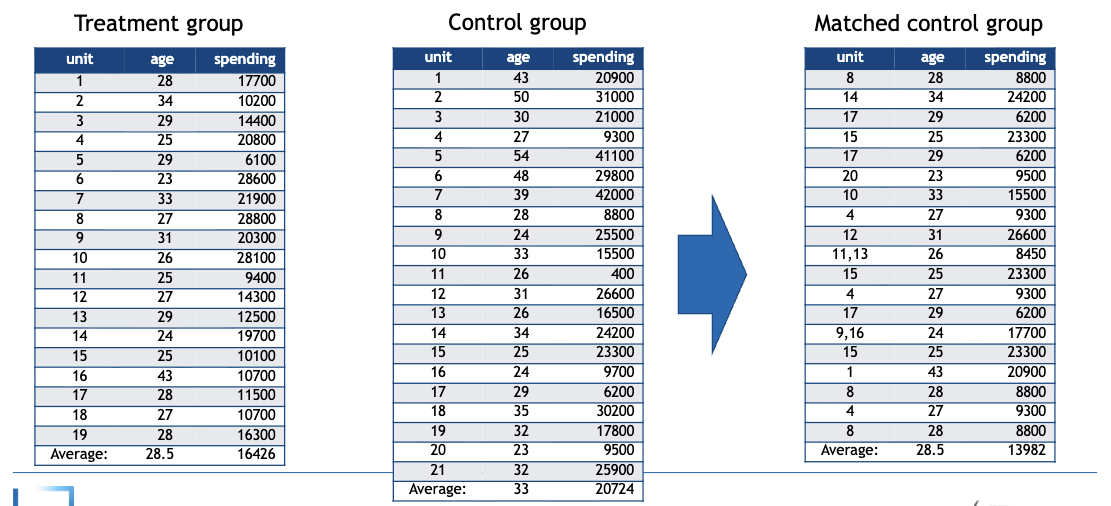
\includegraphics[width=0.8\textwidth]{2026-03-11-19-02-32.png}
\end{figure}
\subsection{Treatment effect estimates}
\begin{itemize}
    \item Differnece in average spending between treatment and control: 
    \begin{itemize}
        \item Before matching: $16426 - 20724 = - 4298$
        \item After matching: $16426 - 13982 = 2444$
    \end{itemize}
    \item The example provides an ATET estimate: we find a match for each treated unit 
    \item We can also use matching to estimate ATE and match in both directions: 
    \begin{itemize}
        \item If observation $i $ is treated, we find matching partners from the untreated/control group
        \item If observation $i $ is untreated, we find matching partners from the treated group
        \item Requires using observation multiple times 
    \end{itemize}
    \item Similarly, we can also focus on ATEU
\end{itemize}
\newpage 
\subsection{Approximate matching}
\begin{itemize}
    \item Exact matches are often not available. In that case, a mathing estimator of ATET can also be constructed as: 
    \begin{gather*}
        \text{ATET} = \frac{1}{N_T}\sum_{W_i}(Y_i - Y_{j(i)})
    \end{gather*}
    wjere $Y_{j(i)} $ is the outcome of an untreated observation such that $X_{j(i)} $ is the closest value to $X_i $ among the untreated observations 
    \item We may also use the average for $M $ closest matches:
    \begin{gather*}
        \text{ATET} = \frac{1}{N_T}\sum_{W_i}\left[Y_i - \left(\frac{1}{M}\sum_{m = 1}^{M}Y_{j_m(i)}\right)\right]
    \end{gather*}
    \item Works very well when we can find good matches for each treated unit, so that $M $ is usually small because there are only few good matches
\end{itemize}
\subsubsection{Bias of approximate matching}
\begin{itemize}
    \item Doing approximate matching will always be biased and may even be inconsistent 
    \item The bias of the matching estimator depends on the matching discrepancies $||X_i - X_{j(i)}|| $
    \item Having multiple matches may reduce variance but increases bias -- bias-variance tradeoff 
    \item There are bias correction techniques that can be applied but they typically have other limitations or strong assuptions 
\end{itemize}
\subsection{Important steps in implementing matching methods}
Matching methods have five key steps: 
\begin{itemize}
    \item Design: 
    \begin{enumerate}
        \item Decide on which covariates $X $ to include 
        \item Defining ``similarity'' or ``closeness''
        \begin{itemize}
            \item Decide on a distance measure to determine similarity
        \end{itemize}
        \item Implementing a matching method, given the similarity measure
        \begin{itemize}
            \item How to assign control units to similar treatment units 
        \end{itemize}
        \item Assessing the quality of matching 
        \begin{itemize}
            \item Potentially iterating between steps 1 and 3 until well-matched sample results 
        \end{itemize}
    \end{enumerate}
    \item Analysis 
    \begin{enumerate}\setcounter{enumi}{4}
        \item Estimate the treatment effect, given the matching done in step 3
    \end{enumerate}
\end{itemize}
\newpage 
\subsubsection{Decide on which covariates to include}
\begin{itemize}
    \item Generally, we should include all pre-treatment covariates that potentially affect the treatment assignment and potential outcomes 
    \begin{itemize}
        \item Some methods pose limitations on the number of variables to include for matching 
        \item Inlcuding irrelevant variables may reduce quality of the matched samples 
    \end{itemize}
    \item We should not include covariates that are affected by the treatment 
\end{itemize}
\subsubsection{Decide on the distance measure}
\begin{itemize}
    \item There are different ways to define the distance $D_{ij} $ between individuals $i\text{ and }j $
    \item Exact matching: 
    \[
    D_{ij} = \begin{cases}
        0 &\text{if }X_i = X_j\\
        \infty &\text{if }X_i \neq X_j
    \end{cases}
    \]
    \begin{itemize}
        \item May require binning or discretization of continuous covariates (e.g., age groups 20-30 etc)
        \item For high dimensional $X $, exact matching often becomes infeasible (curse of dimensionality), and we need to rely on linear transformations of the $X $ into a distance measure 
    \end{itemize}
    \item Mahalanobis: 
    \begin{gather*}
        D_{ij} = \sqrt{(X_i - X_j)'\Sigma^{-1}(X_i - X_j)}
    \end{gather*}
    \begin{itemize}
        \item More common than Euclidian or normed Euclidian distance for matching
        \item Accounts for different variances of $X $ and correlations between $X $
        \item Works best with continuous covariates (assumes normally-, or t-distributed variables)
    \end{itemize}
    \item Other common distance measures, like Manhattan, Chebychev, Euclidian
\end{itemize}
\textbf{Some distance measures}
\begin{figure}[H]
    \centering
    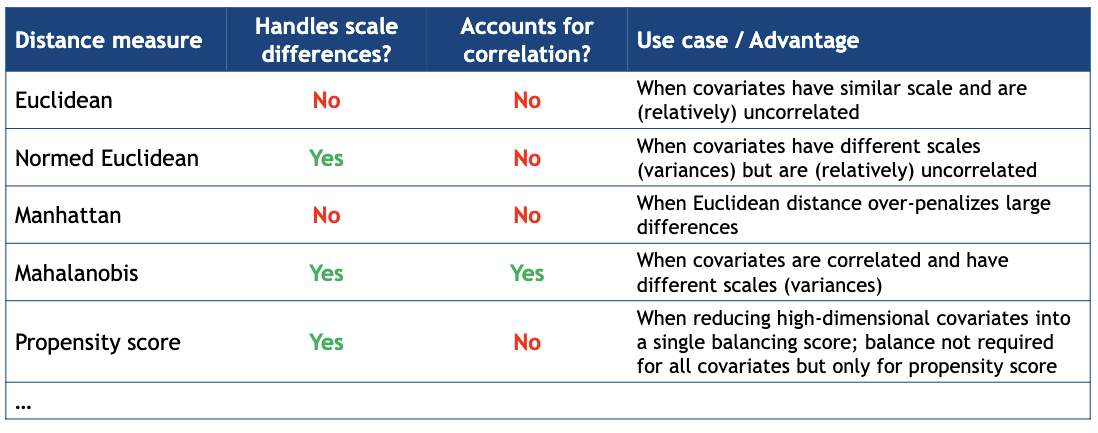
\includegraphics[width=0.8\textwidth]{2026-03-11-19-48-32.png}
\end{figure}
\newpage 
\subsubsection{Implementing the matching method}
\begin{itemize}
    \item Greedy (nearest neighbor) or optimal matching?
    \item With or without replacement?
    \begin{itemize}
        \item Reusing observations for more than one matching partner 
        \item Inference (standard errors) complicated to calculate 
    \end{itemize}
    \item Selecting the number of matches 
    \begin{itemize}
        \item Bias-variance tradeoff: Multiple controls increase bias since the 2nd, 3rd etc. matches are, by definition, further away from the treated individual than it is the 1st closest match. On the other hand, utilizing multiple matches can decrease variance due to the larger matched sample size 
    \end{itemize}
    \item Pruning 
    \begin{itemize}
        \item Defining a maximum distance for matching?
        \item Avoids poor matches that can cause large bias 
        \item Loss of treatment units $\to $ not a true ATET anymore 
    \end{itemize}
    \item \textbf{Choices are interrelated:}
    \begin{itemize}
        \item e.g., greedy is less of a problem when reusing observations (with replacement)
        \item Purining is more important when not reusing observations 
    \end{itemize}
\end{itemize}
\subsubsection{Assessing the quality of matching}
\textbf{Common support / overlap}
\begin{itemize}
    \item Common support is a prerequisite for matching: For every combination of covariates, there exists a positive probability of receiving each treatment level (i.e., there is no combination of covariates that prevents being in treated or untreated condition): $0 < \mathbb{P}[T_i = 1|X_i] < 1 $
    \item We need to observe at least partial overlap of covariate distribution to be able to find matching parners (i.e., there are instances of $X $ in both treatment and untreated condition)
    \begin{figure}[H]
        \centering
        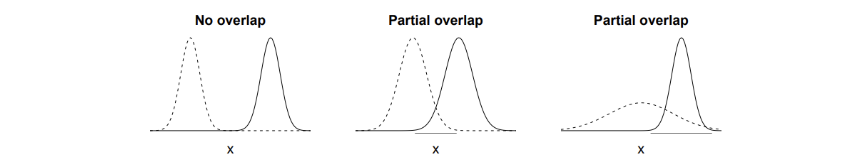
\includegraphics[width=0.8\textwidth]{2026-03-11-19-55-54.png}
    \end{figure}
    \item Depends on whether we try to estimate ATE or ATET 
    \begin{itemize}
        \item For ATET we can discard control units but may not want to discard treatment units 
        \item For ATE we want to keep potentially all units and find a matching parner
    \end{itemize}
\end{itemize}
\newpage 
\subsubsection{Assessing the quality of the matched samples}
\textbf{Covariate balance}
\begin{itemize}
    \item After matching, the covariate distribution in the treated group should not differ from the untreated group 
    \item Exact matching ensures covariate balance; all other methods need to be checked 
    \item Not only equality of means, but also investigate the shape of the distribution (e.g., density histograms)
\end{itemize}
\begin{figure}[H]
    \centering
    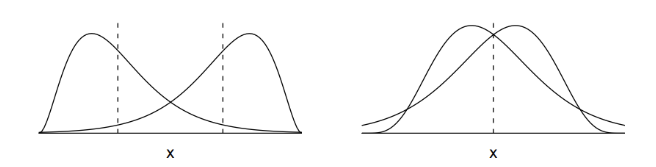
\includegraphics[width=0.8\textwidth]{2026-03-12-08-45-57.png}
\end{figure}
Both imbalance and lack of overlap are also problems for covariate adjustment in OLS regression, but balance may be harder to check than in matching 
\begin{itemize}
    \item OLS does not produce matched treated and untreated groups based on the covariates 
\end{itemize}
\subsection{Decide on the distance measure -- alternatives}
\begin{itemize}
    \item Propensity score matching: 
    \begin{gather*}
        D_{ij} = |p(X_i) - p(X_j)|
    \end{gather*}
    \begin{itemize}
        \item The propensity score measures the probability of being treated conditional on $X $ (next section)
    \end{itemize}
    \item Logit propensity score matching:
    \begin{gather*}
        D_{ij} = \Big|\text{logit}\big(p(X_i)\big) - \text{logit}\big(p(X_j)\big)\Big|
    \end{gather*}
    \begin{itemize}
        \item May provide better matching results than using propensity scores directly by ensuring that small differences in extreme propensity scores (close to 1 or 0) are deemphasized
    \end{itemize}
    \item Combinations of exact matching and propensity score matching 
    \begin{itemize}
        \item Match on specific important covariates directly (e.g., loyalty card member)
        \item Match within these strata using propensity score matching 
    \end{itemize}
\end{itemize}
\newpage 
\section{Propensity scores}
\subsection{The core idea}
\begin{itemize}
    \item The propensity score measures the probability of being treated conditional on $X $
    \begin{gather*}
        p(X_i) = \mathbb{P}[T_i = 1|X_i]
    \end{gather*}
    \item In an ideal randomized experiment with two arms (i.e., $T_i\in \{0, 1\}$) and equal group sizes, the propensity score is constant at 0.5
    \begin{itemize}
        \item More generally, for randomized $T_i $, we have $p(X_i) = p_0\in \{0, 1\} $
    \end{itemize}
    \item However,
    \begin{itemize}
        \item We do not know the actual propensity scores $p(X_i) $ but can only estimate $\hat{p}(X_i) $
        \item In practice, the $\hat{p}(X_i) $ is rarely constant even for randomized experiments because covariate distribution is rarely perfect in finite samples 
        \item Looking at the distribution/variability of the $\hat{p}(X_i) $, gives a measure of how far we are from a randomized experiment given the covariates 
    \end{itemize}
    \item Propensity scores are a great way to reduce the dimensionality of $X $ because they have some nice properties 
    \item Given the ``selection on observables'' (conditional independence) assumption: 
    \begin{gather*}
        \{Y_i(1), Y_i(0)\} \bot T_i|X_i
    \end{gather*}
    \item Plus ``common support'' 
    \begin{gather*}
        0 < \mathbb{P}[T_i = 1 | X_i] < 1
    \end{gather*}
    \item Rosenbaum shows that this implies:
    \begin{gather*}
        \{Y_i(1), Y_i(0)\} \bot T_i|p(X_i)
    \end{gather*}
    \begin{itemize}
        \item Conditioning on the propensity score is enough to have independence between the treatment indicator and the potential outcomes 
        \item If we are able to find exact matches in propensity scores, we have an unbiased estimator 
    \end{itemize}
\end{itemize}
\newpage 
\subsection{Balancing properly}
\begin{itemize}
    \item $T\text{ and } X $ are independent conditional on $p(X):\, X_i\bot T_i|p(X_i) $
    \begin{itemize}
        \item Because $p(X) $ explains the selection mechanism into $T \text{ given } X $
    \end{itemize}
    \item Thus, we obtain the balancing propery of ther propensity score: 
    \begin{gather*}
        \mathbb{P}\big(X_i|T_i = 1,\, p(X_i)\big) = \mathbb{P}\big(X_i|T_i = 0,\, p(X_i)\big) 
    \end{gather*}
    \begin{itemize}
        \item Conditional on the propensity score, the distribution of the covariates is the same for treated and untreated individuals
    \end{itemize}
    \item We can use this to check if our estimated propensity score actually produces balance:
    \begin{gather*}
        \mathbb{P}\big(X_i|T_i = 1,\, \hat{p}(X_i)\big) = \mathbb{P}\big(X_i|T_i = 0,\, \hat{p}(X_i)\big) 
    \end{gather*} 
\end{itemize}
\subsection{How to estimate the propensity score?}
\begin{itemize}
    \item Most commonly the propensity score $\hat{p}(X_i) $ is estimated through logistic regression 
    \begin{itemize}
        \item Limitations: specific functional form and parametric method 
    \end{itemize}
    \item Estimating the propensity score $\hat{p}(X_i) $ is a standard prediction problem for which we may use any nonparametric ML approach
    \begin{itemize}
        \item e.g., classification trees, random forests, gradient boosting etc. 
        \item Requires measures to reduce overfitting
        \item However, the predictive quality of the propensity score does not necessarily translate into its balancing properties; some research shows that fancy ML methods may not be better (but worse) than old-school logistic regression in reducing the confounding bias 
    \end{itemize}
    \item The task is not to best predict assignment, but to control for (include) only those variables that are predicting assignment and outcome (i.e., confounders)
    \begin{itemize}
        \item Those that we need for conditional independence
    \end{itemize}
\end{itemize}
\newpage 
\section{Weighting}
\textbf{Weighting vs. matching}
\begin{figure}[H]
    \centering
    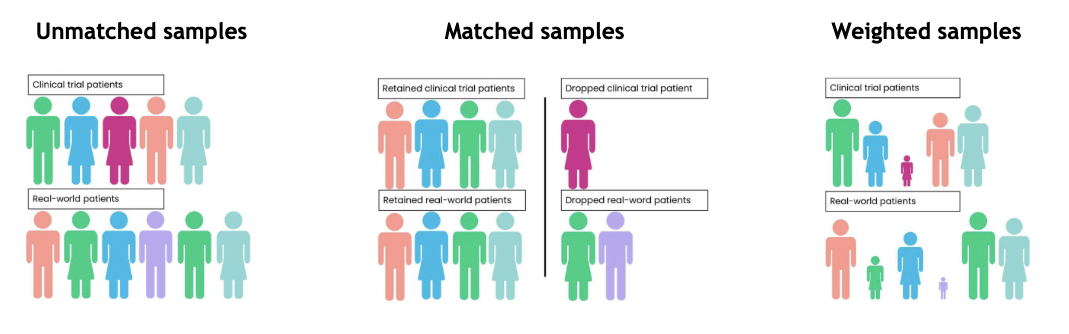
\includegraphics[width=1\textwidth]{2026-03-12-09-13-38.png}
\end{figure}
\subsection{Inverse propensity weighting (IPW)}
\begin{itemize}
    \item Under the previous assumption $\{Y_i(1)- Y_i(0)\} \bot T_i|X_i $ implying $\{Y_i(1) - Y_i(0)\} \bot T_i|p(X_i) $
    \item The ATE can also be consistently estimated as 
    \begin{gather*}
        \text{ATE} = \mathbb{E}[Y_i(1) - Y_i(0)] = \mathbb{E}\left[\frac{T_i}{p(X_i)}Y_i - \frac{(1 - T_i)}{1 - p(X_i)}\right] = \mathbb{E}\left[Y_i \frac{T_i - p(X_i)}{p(X_i)(1 - p(X_i))}\right]
    \end{gather*}
    \item Thus, given the estimated propensity scores $\hat{p}(X_i)$ for each individual, we can construct the so-called \textbf{inverse propensity weighted (IPW)} estimator $\hat{\tau}_{\text{IPW}} $
    \begin{gather*}
        \hat{\tau}_{\text{IPW}} = \frac{1}{N} \sum_{i = 1}^{N}\left[Y_i\left(\frac{T_i}{\hat{p}(X_i)} - \frac{(1 - T_i)}{1 - \hat{p}(X_i)}\right)\right] = \frac{1}{N}\sum_{i = 1}^{N}\left[Y_i \frac{T_i - \hat{p}(X_i)}{\hat{p}(X_i)(1 - \hat{p}(X_i))}\right]
    \end{gather*}
    \begin{itemize}
        \item Weights up (or down) the over-represented (or under-represented) observations 
    \end{itemize}
\end{itemize}
\newpage 
\subsection{Propensity score weighting -- numerical examples}
\begin{figure}[H]
    \centering
    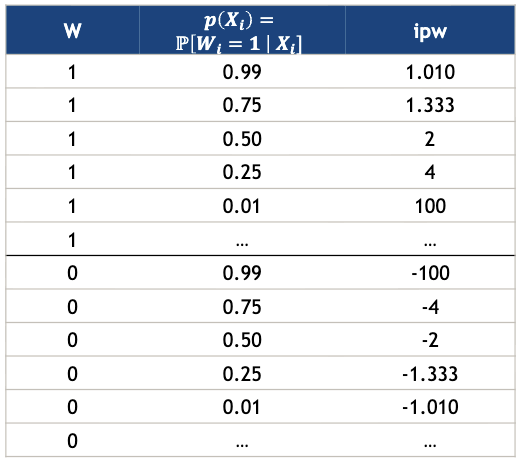
\includegraphics[width=0.5\textwidth]{2026-03-12-09-23-20.png}
\end{figure}
\begin{itemize}
    \item Large propensity score and treated $(T = 1) $
    \begin{itemize}
        \item The likelihood is high that those observations got treatment based on the $X $ and thus do not need (much) reweighting
        \item Low weight (close to one)
    \end{itemize}
    \item Low propensity score and treated $(T = 1) $
    \begin{itemize}
        \item The likelihood is low that those observations got treatment based on the $X $ (we have only few examples in the data) and thus these need reweighting (need to get a larger weight to make the overall sample balanced)
        \item Large weight 
    \end{itemize}
    \item Vice versa for untreated 
\end{itemize}
\subsection{Issues with propensity score weighting}
\begin{itemize}
    \item Core issue with matching estimators remains: require balance and overlap 
    \item IPW has an inherent balancing property, but still requires overlap in the propensity score distribution
    \item When overlap is weak, models rely on extrapolation in regions where data are sparse 
    \item Large variance: the estimator typically has quite large variance and is not very stable 
\end{itemize}
\newpage 
\subsection{Doubly robust estimators (AIPW)}
\begin{itemize}
    \item Combines propensity score based and regression-based estimation 
    \item Estimators that only need the propensity score OR the regression function to be correctly specified: the augmented IPW estimator (AIPW)
    \begin{gather*}
        \text{ATE} = \frac{1}{N}\sum_{i = 1}^{N}\left(\frac{T_i}{\hat{p}(X_i)}\left(Y_i - \hat{\mu}_{T = 1}(X_i)\right) + \hat{\mu}_{T = 1}(X_i)\right) - \frac{1}{N}\sum_{i = 1}^{N}\left(\frac{(1 - T_i)}{1 - \hat{p}(X_i)}\left(Y_i - \hat{\mu}_{T = 0}(X_i)\right) + \hat{\mu}_{T = 0}(X_i)\right)
    \end{gather*}
    \begin{itemize}
        \item With $\hat{\mu}_{T = 1}(X_i)\text{ and }\hat{\mu}_{T = 0}(X_i) $ being the predicted value from a regression of $X \text{ on }Y $ for only treated or untreated observations 
    \end{itemize}
    \item Typical way to estimate standard errors / confidence intervals: bootstrap
    \item To better understand: rewrite in two parts:
    \begin{gather*}
        \text{ATE} = \underset{\text{Simple regression adjustment}}{\underbrace{\frac{1}{N}\sum_{i = 1}^{N}\left(\hat{\mu}_{T = 1}(X_i) - \hat{\mu}_{T = 0}(X_i)\right)}} + \underset{\text{IPW estimator on the residuals of the regression model $Y_i - \hat{\mu}(X_i) $}}{\underbrace{\frac{1}{N}\sum_{i = 1}^{N}\left(\frac{T_i}{\hat{p}(X_i)}\left(Y_i - \hat{\mu}_{T = 1}(X_i)\right) - \frac{(1 - T_i)}{1 - \hat{p}(X_i)}\left(Y_i - \hat{\mu}_{T = 0}(X_i)\right)\right)}}
    \end{gather*}
    \item If the regression model is correct, then $\mathbb{E}[Y_i - \hat{\mu}(X_i)|X_i] $ will be zero and the second part vanishes (i.e., we don't need the second part, because the first is already giving the right estimate)
    \item If the regression model is not correct, but the propensity score model is, the second part will properly correct (debias) the regression model estimates using the residuals 
    \item However, $\hat{\mu}_{T = 1}(X_i)\text{ and }\hat{\mu}_{T = 0}(X_i) $ must not come from an OLS regression
\end{itemize}
\subsection{Characteristics of the AIPW model}
\begin{itemize}
    \item Model misspecification
    \begin{itemize}
        \item The estimator is doubly robust: it requires only one of the two models -- propensity score model or outcome model to be correct 
        \item However, if both are wrong, the bias can be larger than in any of the two separately 
    \end{itemize}
    \item Variance and instability in small samples 
    \begin{itemize}
        \item Usually, AIPW has smaller variance than the IPW estimator 
        \item If the outcome model is overfitted, it can lead to poor generalization
    \end{itemize}
\end{itemize}

\end{document}